\section{Reagents}
Sometimes called \emph{Materials and chemicals}.

State the type and characteristics of the reagents used: always give the concentration of solutions and, for solids, the purity grade. When a safety data sheet (SDS) is available, summarise its key information: pictograms, H and P statements, personal protective equipment (PPE) and occupational exposure limits.

Chemical formulae are written with the \texttt{mhchem} package and quantities with \texttt{siunitx}:
\begin{itemize}
    \item \ce{H3PO4}, \qty{0.3}{\mole\per\litre}, \qty{25}{\milli\litre};
    \item \ce{H2O2}, \qty{30}{\percent} (w/w), \qty{10}{\milli\litre}.
\end{itemize}

\Cref{tab:reagents} shows a compact safety table; the P statements are written as codes and can be listed in full at the end of the report.

\begin{table}[ht]
    \centering
    \footnotesize
    \begin{tabularx}{\textwidth}{C{0.12\textwidth} C{0.14\textwidth} >{\raggedright\arraybackslash}X C{0.16\textwidth} C{0.12\textwidth}}
        \toprule
        \textbf{Compound} & \textbf{Structure} & \textbf{H and P statements} & \textbf{Pictograms} & \textbf{PPE} \\
        \midrule
        \ce{H2O2}
         & 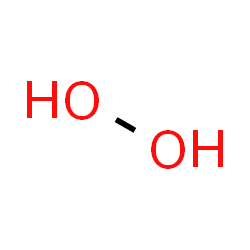
\includegraphics[width=0.12\textwidth]{img/hydrogen_peroxide.png}
         & H: H271, H302, H314, H332.\newline
        P: P210, P220, P221, P260, P261, P264, P270, P271, P280, P283, P301+P312, P301+P330+P331, P303+P361+P353, P304+P312, P304+P340, P305+P351+P338, P306+P360, P310, P312, P321, P330, P363, P370+P378, P371+P380+P375, P405, P501.
         & 
\includegraphics[width=0.07\textwidth]{img/pictograms/oxidizing.png}
        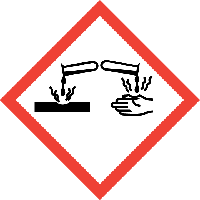
\includegraphics[width=0.07\textwidth]{img/pictograms/corrosive.png}\newline
        
\includegraphics[width=0.07\textwidth]{img/pictograms/health-hazard.png}
         & gloves, goggles, face shield \\
        \bottomrule
    \end{tabularx}
    \caption{Chemicals used in the experiment. The H and P statements are given in full at the end of the report.}
    \label{tab:reagents}
\end{table}

\Cref{tab:reagents-tlv} extends the previous table with the occupational exposure limits: concentrations of airborne substances below which most workers can be exposed repeatedly, day after day, without adverse health effects. The commands \verb|\Hphrase| and \verb|\Pphrase| print the full text of each statement.

\begin{table}[ht]
    \centering
    \footnotesize
    \begin{tabularx}{\textwidth}{C{0.12\textwidth} C{0.10\textwidth} >{\raggedright\arraybackslash}X C{0.13\textwidth} C{0.10\textwidth} C{0.09\textwidth}}
        \toprule
        \textbf{Compound} & \textbf{Structure} & \textbf{H and P statements} & \textbf{Pictograms} & \textbf{PPE} & \textbf{Limits [ppm]} \\
        \midrule
        \ce{H2O2}
         & 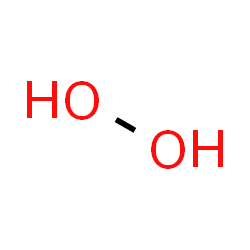
\includegraphics[width=0.09\textwidth]{img/hydrogen_peroxide.png}
         & \Hphrase{H271}\newline \Hphrase{H302}\newline \Hphrase{H314}\newline \Hphrase{H332}\newline \Pphrase{P280}\newline \Pphrase{P305+P351+P338}
         & 
\includegraphics[width=0.07\textwidth]{img/pictograms/oxidizing.png}\newline
        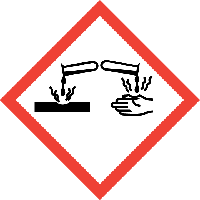
\includegraphics[width=0.07\textwidth]{img/pictograms/corrosive.png}\newline
        
\includegraphics[width=0.07\textwidth]{img/pictograms/health-hazard.png}
         & gloves, goggles, face shield
         & LTEL: 1\newline STEL: 2 \\
        \bottomrule
    \end{tabularx}
    \caption{Chemicals used in the experiment with their exposure limits. LTEL: long-term exposure limit (8-hour time-weighted average); STEL: short-term exposure limit (15 minutes).}
    \label{tab:reagents-tlv}
\end{table}

For syntheses a different table is often more useful (\cref{tab:synthesis}): it collects stoichiometric ratios, masses and yields, which help to follow the mechanism when it depends on the reagent quantities.

\begin{table}[ht]
    \centering
    \footnotesize
    \setlength{\tabcolsep}{3pt}
    \begin{tabularx}{\textwidth}{*{9}{>{\centering\arraybackslash}X}}
        \toprule
        Substance & Molar mass [\unit{\gram\per\mole}] & Amount [\unit{\mole}] & Stoich.\ ratio & Mass [\unit{\gram}] & Volume [\unit{\milli\litre}] & Yield [\unit{\percent}] & H statements & P statements \\
        \midrule
        A         & B                                  & C                     & D              & E                 & F                            & G                       & H            & I            \\
        \bottomrule
    \end{tabularx}
    \caption{Table for syntheses.}
    \label{tab:synthesis}
\end{table}

\begin{table}[ht]
    \centering
    \footnotesize
    \begin{tabularx}{\textwidth}{*{7}{>{\raggedright\arraybackslash}X}}
        \toprule
        Compound  & Structure & Appearance       & Hazards & Protection & TLV/TWA    & Disposal     \\
        \midrule
        \ce{H2O}  &           & colourless liquid & none   & none       & not relevant & down the sink \\
        \ce{NaCl} &           & white solid       & none   & none       & not relevant & down the sink \\
        \bottomrule
    \end{tabularx}
    \caption{Another reagent table layout.}
    \label{tab:reagents-alt}
\end{table}

To find the PPE, search the web for the compound name followed by \enquote{safety data sheet} and use the most recent result.
\info[inline]{Example: \enquote{benzoic acid safety data sheet}.}

Note the manufacturer of each reagent (a photo of the bottle in the lab is enough): it speeds up the search and makes the data more accurate, since sheets from different suppliers may differ. Besides the PPE, the SDS contains much more useful information.
